\subsection{Abbildungen}\label{subsec:abbildungen}

	\bigskip\noindent
	\begin{minipage}{\textwidth}
		\centering
		\captionof{figure}{Beispiel SOAP-Kommunikation}
		\label{fig:soapKommunikation}
		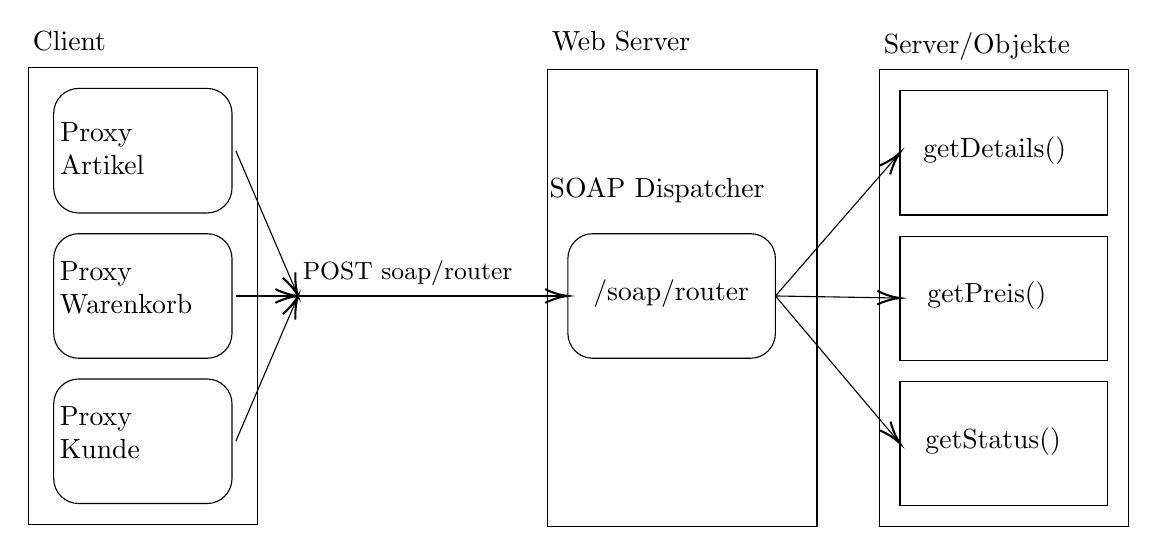
\begin{tikzpicture}[x=0.75pt,y=0.75pt,yscale=-1,xscale=1]
%uncomment if require: \path (0,300); %set diagram left start at 0, and has height of 300

%Shape: Rectangle [id:dp6713021135531445] 
	\draw   (20,40) -- (130.45,40) -- (130.45,260) -- (20,260) -- cycle ;
%Shape: Rectangle [id:dp9488356654027563] 
	\draw   (270,41) -- (400,41) -- (400,261) -- (270,261) -- cycle ;
%Shape: Rectangle [id:dp051438042119226646] 
	\draw   (430,41) -- (550,41) -- (550,261) -- (430,261) -- cycle ;
%Rounded Rect [id:dp025938333082131892] 
	\draw   (32.27,62) .. controls (32.27,55.37) and (37.65,50) .. (44.27,50) -- (106.18,50) .. controls (112.81,50) and (118.18,55.37) .. (118.18,62) -- (118.18,98) .. controls (118.18,104.63) and (112.81,110) .. (106.18,110) -- (44.27,110) .. controls (37.65,110) and (32.27,104.63) .. (32.27,98) -- cycle ;
%Rounded Rect [id:dp6746062988145041] 
	\draw   (32.27,132) .. controls (32.27,125.37) and (37.65,120) .. (44.27,120) -- (106.18,120) .. controls (112.81,120) and (118.18,125.37) .. (118.18,132) -- (118.18,168) .. controls (118.18,174.63) and (112.81,180) .. (106.18,180) -- (44.27,180) .. controls (37.65,180) and (32.27,174.63) .. (32.27,168) -- cycle ;
%Rounded Rect [id:dp3846676301494929] 
	\draw   (32.27,202) .. controls (32.27,195.37) and (37.65,190) .. (44.27,190) -- (106.18,190) .. controls (112.81,190) and (118.18,195.37) .. (118.18,202) -- (118.18,238) .. controls (118.18,244.63) and (112.81,250) .. (106.18,250) -- (44.27,250) .. controls (37.65,250) and (32.27,244.63) .. (32.27,238) -- cycle ;
%Rounded Rect [id:dp803526501517456] 
	\draw   (280,132) .. controls (280,125.37) and (285.37,120) .. (292,120) -- (368,120) .. controls (374.63,120) and (380,125.37) .. (380,132) -- (380,168) .. controls (380,174.63) and (374.63,180) .. (368,180) -- (292,180) .. controls (285.37,180) and (280,174.63) .. (280,168) -- cycle ;
%Shape: Rectangle [id:dp10324218660152407] 
	\draw   (440,51) -- (540,51) -- (540,111) -- (440,111) -- cycle ;
%Shape: Rectangle [id:dp9289733601126315] 
	\draw   (440,121.5) -- (540,121.5) -- (540,181) -- (440,181) -- cycle ;
%Shape: Rectangle [id:dp060786979153347964] 
	\draw   (440,191) -- (540,191) -- (540,251) -- (440,251) -- cycle ;
%Straight Lines [id:da4074949520827229] 
	\draw    (150,150) -- (278,150) ;
	\draw [shift={(280,150)}, rotate = 180] [color={rgb, 255:red, 0; green, 0; blue, 0 }  ][line width=0.75]    (10.93,-3.29) .. controls (6.95,-1.4) and (3.31,-0.3) .. (0,0) .. controls (3.31,0.3) and (6.95,1.4) .. (10.93,3.29)   ;
%Straight Lines [id:da18649676798360515] 
	\draw    (380,150) -- (438.69,82.51) ;
	\draw [shift={(440,81)}, rotate = 491.01] [color={rgb, 255:red, 0; green, 0; blue, 0 }  ][line width=0.75]    (10.93,-3.29) .. controls (6.95,-1.4) and (3.31,-0.3) .. (0,0) .. controls (3.31,0.3) and (6.95,1.4) .. (10.93,3.29)   ;
%Straight Lines [id:da882291870882637] 
	\draw    (380,150) -- (438,150.97) ;
	\draw [shift={(440,151)}, rotate = 180.95] [color={rgb, 255:red, 0; green, 0; blue, 0 }  ][line width=0.75]    (10.93,-3.29) .. controls (6.95,-1.4) and (3.31,-0.3) .. (0,0) .. controls (3.31,0.3) and (6.95,1.4) .. (10.93,3.29)   ;
%Straight Lines [id:da06798859261533052] 
	\draw    (380,150) -- (438.71,219.47) ;
	\draw [shift={(440,221)}, rotate = 229.8] [color={rgb, 255:red, 0; green, 0; blue, 0 }  ][line width=0.75]    (10.93,-3.29) .. controls (6.95,-1.4) and (3.31,-0.3) .. (0,0) .. controls (3.31,0.3) and (6.95,1.4) .. (10.93,3.29)   ;
%Straight Lines [id:da09553391086743068] 
	\draw    (120,80) -- (149.21,148.16) ;
	\draw [shift={(150,150)}, rotate = 246.8] [color={rgb, 255:red, 0; green, 0; blue, 0 }  ][line width=0.75]    (10.93,-3.29) .. controls (6.95,-1.4) and (3.31,-0.3) .. (0,0) .. controls (3.31,0.3) and (6.95,1.4) .. (10.93,3.29)   ;
%Straight Lines [id:da8931516225216165] 
	\draw    (120,220) -- (149.21,151.84) ;
	\draw [shift={(150,150)}, rotate = 473.2] [color={rgb, 255:red, 0; green, 0; blue, 0 }  ][line width=0.75]    (10.93,-3.29) .. controls (6.95,-1.4) and (3.31,-0.3) .. (0,0) .. controls (3.31,0.3) and (6.95,1.4) .. (10.93,3.29)   ;
%Straight Lines [id:da2835861250266003] 
	\draw    (120,150) -- (148,150) ;
	\draw [shift={(150,150)}, rotate = 180] [color={rgb, 255:red, 0; green, 0; blue, 0 }  ][line width=0.75]    (10.93,-3.29) .. controls (6.95,-1.4) and (3.31,-0.3) .. (0,0) .. controls (3.31,0.3) and (6.95,1.4) .. (10.93,3.29)   ;

% Text Node
	\draw (21,21) node [anchor=north west][inner sep=0.75pt]   [align=left] {Client};
% Text Node
	\draw (271,21) node [anchor=north west][inner sep=0.75pt]   [align=left] {Web Server};
% Text Node
	\draw (431,22) node [anchor=north west][inner sep=0.75pt]   [align=left] {Server/Objekte};
% Text Node
	\draw (34.27,65) node [anchor=north west][inner sep=0.75pt]   [align=left] {Proxy\\Artikel};
% Text Node
	\draw (34,132) node [anchor=north west][inner sep=0.75pt]   [align=left] {Proxy \\Warenkorb};
% Text Node
	\draw (34,202) node [anchor=north west][inner sep=0.75pt]   [align=left] {Proxy \\Kunde};
% Text Node
	\draw (291,141) node [anchor=north west][inner sep=0.75pt]   [align=left] {/soap/router};
% Text Node
	\draw (450,72) node [anchor=north west][inner sep=0.75pt]   [align=left] {getDetails()};
% Text Node
	\draw (452,142) node [anchor=north west][inner sep=0.75pt]   [align=left] {getPreis()};
% Text Node
	\draw (451,212) node [anchor=north west][inner sep=0.75pt]   [align=left] {getStatus()};
% Text Node
	\draw (151,132) node [anchor=north west][inner sep=0.75pt]  [font=\small] [align=left] {POST soap/router};
% Text Node
	\draw (270,92) node [anchor=north west][inner sep=0.75pt]   [align=left] {SOAP Dispatcher};


\end{tikzpicture}

	\end{minipage}

	\bigskip\noindent
	\begin{minipage}{\textwidth}
		\centering
		\captionof{figure}{Beispiel REST-Kommunikation}
		\label{fig:restKommunikation}
		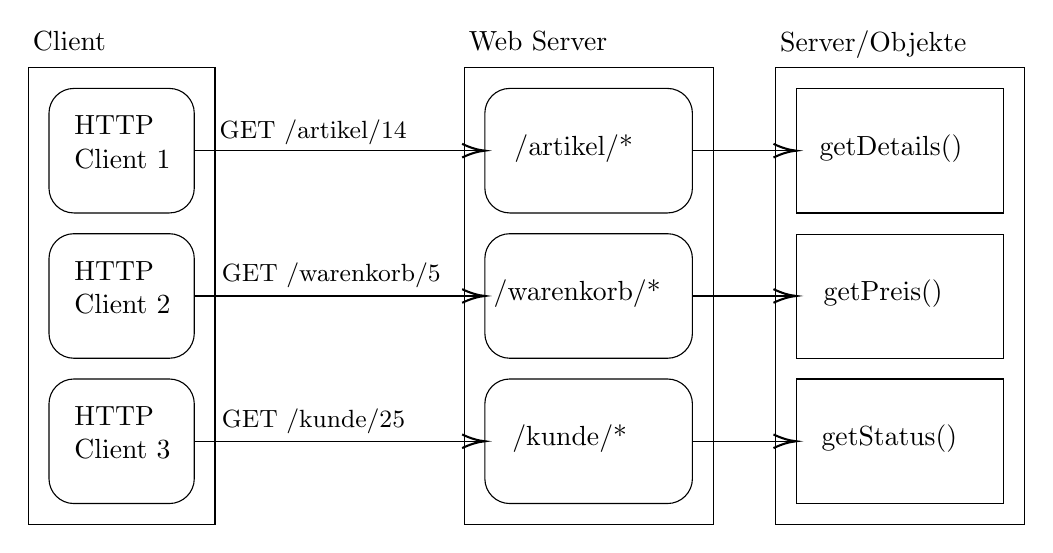
\begin{tikzpicture}[x=0.75pt,y=0.75pt,yscale=-1,xscale=1]
%uncomment if require: \path (0,300); %set diagram left start at 0, and has height of 300

%Shape: Rectangle [id:dp6713021135531445]
	\draw   (20,40) -- (110,40) -- (110,260) -- (20,260) -- cycle ;
%Shape: Rectangle [id:dp9488356654027563]
	\draw   (230,40) -- (350,40) -- (350,260) -- (230,260) -- cycle ;
%Shape: Rectangle [id:dp051438042119226646]
	\draw   (380,40) -- (500,40) -- (500,260) -- (380,260) -- cycle ;
%Rounded Rect [id:dp025938333082131892]
	\draw   (30,62) .. controls (30,55.37) and (35.37,50) .. (42,50) -- (88,50) .. controls (94.63,50) and (100,55.37) .. (100,62) -- (100,98) .. controls (100,104.63) and (94.63,110) .. (88,110) -- (42,110) .. controls (35.37,110) and (30,104.63) .. (30,98) -- cycle ;
%Rounded Rect [id:dp6746062988145041]
	\draw   (30,132) .. controls (30,125.37) and (35.37,120) .. (42,120) -- (88,120) .. controls (94.63,120) and (100,125.37) .. (100,132) -- (100,168) .. controls (100,174.63) and (94.63,180) .. (88,180) -- (42,180) .. controls (35.37,180) and (30,174.63) .. (30,168) -- cycle ;
%Rounded Rect [id:dp3846676301494929]
	\draw   (30,202) .. controls (30,195.37) and (35.37,190) .. (42,190) -- (88,190) .. controls (94.63,190) and (100,195.37) .. (100,202) -- (100,238) .. controls (100,244.63) and (94.63,250) .. (88,250) -- (42,250) .. controls (35.37,250) and (30,244.63) .. (30,238) -- cycle ;
%Rounded Rect [id:dp5291262901539]
	\draw   (240,62) .. controls (240,55.37) and (245.37,50) .. (252,50) -- (328,50) .. controls (334.63,50) and (340,55.37) .. (340,62) -- (340,98) .. controls (340,104.63) and (334.63,110) .. (328,110) -- (252,110) .. controls (245.37,110) and (240,104.63) .. (240,98) -- cycle ;
%Rounded Rect [id:dp803526501517456]
	\draw   (240,132) .. controls (240,125.37) and (245.37,120) .. (252,120) -- (328,120) .. controls (334.63,120) and (340,125.37) .. (340,132) -- (340,168) .. controls (340,174.63) and (334.63,180) .. (328,180) -- (252,180) .. controls (245.37,180) and (240,174.63) .. (240,168) -- cycle ;
%Rounded Rect [id:dp4732941799846049]
	\draw   (240,202) .. controls (240,195.37) and (245.37,190) .. (252,190) -- (328,190) .. controls (334.63,190) and (340,195.37) .. (340,202) -- (340,238) .. controls (340,244.63) and (334.63,250) .. (328,250) -- (252,250) .. controls (245.37,250) and (240,244.63) .. (240,238) -- cycle ;
%Shape: Rectangle [id:dp10324218660152407]
	\draw   (390,50) -- (490,50) -- (490,110) -- (390,110) -- cycle ;
%Shape: Rectangle [id:dp9289733601126315]
	\draw   (390,120.5) -- (490,120.5) -- (490,180) -- (390,180) -- cycle ;
%Shape: Rectangle [id:dp060786979153347964]
	\draw   (390,190) -- (490,190) -- (490,250) -- (390,250) -- cycle ;
%Straight Lines [id:da4074949520827229]
	\draw    (100,80) -- (238,80) ;
	\draw [shift={(240,80)}, rotate = 180] [color={rgb, 255:red, 0; green, 0; blue, 0 }  ][line width=0.75]    (10.93,-3.29) .. controls (6.95,-1.4) and (3.31,-0.3) .. (0,0) .. controls (3.31,0.3) and (6.95,1.4) .. (10.93,3.29)   ;
%Straight Lines [id:da7678440087120453]
	\draw    (100,150) -- (238,150) ;
	\draw [shift={(240,150)}, rotate = 180] [color={rgb, 255:red, 0; green, 0; blue, 0 }  ][line width=0.75]    (10.93,-3.29) .. controls (6.95,-1.4) and (3.31,-0.3) .. (0,0) .. controls (3.31,0.3) and (6.95,1.4) .. (10.93,3.29)   ;
%Straight Lines [id:da8610972651984123]
	\draw    (100,220) -- (238,220) ;
	\draw [shift={(240,220)}, rotate = 180] [color={rgb, 255:red, 0; green, 0; blue, 0 }  ][line width=0.75]    (10.93,-3.29) .. controls (6.95,-1.4) and (3.31,-0.3) .. (0,0) .. controls (3.31,0.3) and (6.95,1.4) .. (10.93,3.29)   ;
%Straight Lines [id:da18649676798360515]
	\draw    (340,80) -- (388,80) ;
	\draw [shift={(390,80)}, rotate = 180] [color={rgb, 255:red, 0; green, 0; blue, 0 }  ][line width=0.75]    (10.93,-3.29) .. controls (6.95,-1.4) and (3.31,-0.3) .. (0,0) .. controls (3.31,0.3) and (6.95,1.4) .. (10.93,3.29)   ;
%Straight Lines [id:da882291870882637]
	\draw    (340,150) -- (388,150) ;
	\draw [shift={(390,150)}, rotate = 180] [color={rgb, 255:red, 0; green, 0; blue, 0 }  ][line width=0.75]    (10.93,-3.29) .. controls (6.95,-1.4) and (3.31,-0.3) .. (0,0) .. controls (3.31,0.3) and (6.95,1.4) .. (10.93,3.29)   ;
%Straight Lines [id:da06798859261533052]
	\draw    (340,220) -- (388,220) ;
	\draw [shift={(390,220)}, rotate = 180] [color={rgb, 255:red, 0; green, 0; blue, 0 }  ][line width=0.75]    (10.93,-3.29) .. controls (6.95,-1.4) and (3.31,-0.3) .. (0,0) .. controls (3.31,0.3) and (6.95,1.4) .. (10.93,3.29)   ;

% Text Node
	\draw (21,21) node [anchor=north west][inner sep=0.75pt]   [align=left] {Client};
% Text Node
	\draw (231,21) node [anchor=north west][inner sep=0.75pt]   [align=left] {Web Server};
% Text Node
	\draw (381,21) node [anchor=north west][inner sep=0.75pt]   [align=left] {Server/Objekte};
% Text Node
	\draw (41,62) node [anchor=north west][inner sep=0.75pt]   [align=left] {HTTP \\Client 1};
% Text Node
	\draw (41,132) node [anchor=north west][inner sep=0.75pt]   [align=left] {HTTP \\Client 2};
% Text Node
	\draw (41,202) node [anchor=north west][inner sep=0.75pt]   [align=left] {HTTP \\Client 3};
% Text Node
	\draw (253,71) node [anchor=north west][inner sep=0.75pt]   [align=left] {/artikel/*};
% Text Node
	\draw (243,141) node [anchor=north west][inner sep=0.75pt]   [align=left] {/warenkorb/*};
% Text Node
	\draw (252,211) node [anchor=north west][inner sep=0.75pt]   [align=left] {/kunde/*};
% Text Node
	\draw (400,71) node [anchor=north west][inner sep=0.75pt]   [align=left] {getDetails()};
% Text Node
	\draw (402,141) node [anchor=north west][inner sep=0.75pt]   [align=left] {getPreis()};
% Text Node
	\draw (401,211) node [anchor=north west][inner sep=0.75pt]   [align=left] {getStatus()};
% Text Node
	\draw (112,133) node [anchor=north west][inner sep=0.75pt]  [font=\small] [align=left] {GET /warenkorb/5};
% Text Node
	\draw (112,203) node [anchor=north west][inner sep=0.75pt]  [font=\small] [align=left] {GET /kunde/25};
% Text Node
	\draw (111,64) node [anchor=north west][inner sep=0.75pt]  [font=\small] [align=left] {GET /artikel/14};


\end{tikzpicture}

	\end{minipage}

	\bigskip\noindent
	\begin{minipage}{\textwidth}
		\centering
		\captionof{figure}{Schichtenmodell}
		\label{fig:schichtenmodell}
		\input{include/tikzDiagrams/Schichtenmodell.tikz}
	\end{minipage}

	\bigskip\noindent
	\begin{minipage}{\textwidth}
		\centering
		\captionof{figure}[OAuth 2.0 Abstrakter Protokoll Fluss]
		{OAuth 2.0 Abstrakter Protokoll Fluss\\Quelle:~\fullcite{rfc6749}}
		\label{fig:oauthAbstractFlow}
		\input{include/tikzDiagrams/OAuthAbstractWorkFlow.tikz}
	\end{minipage}

	\bigskip\noindent
	\begin{minipage}{\textwidth}
		\centering
		\captionof{figure}[OpenID Connect Core Abstrakter Protokoll Fluss]
		{OpenID Connect Core Abstrakter Protokoll Fluss\\Quelle:~\fullcite{oidc}}
		\label{fig:openIDAbstractFlow}
		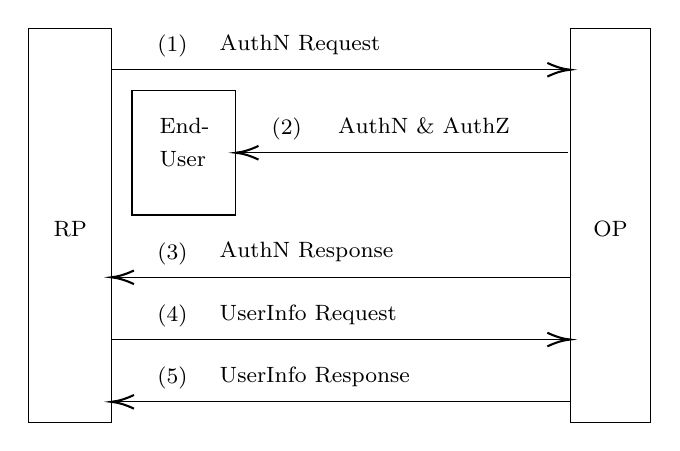
\begin{tikzpicture}[x=0.75pt,y=0.75pt,yscale=-1,xscale=1]
%uncomment if require: \path (0,241); %set diagram left start at 0, and has height of 241

%Shape: Rectangle [id:dp07154197464055945]
	\draw   (10,10) -- (50,10) -- (50,200) -- (10,200) -- cycle ;
%Shape: Rectangle [id:dp5402475504345341]
	\draw   (271.05,10) -- (310,10) -- (310,200) -- (271.05,200) -- cycle ;
%Straight Lines [id:da14410399364813653]
	\draw    (50,30) -- (269.05,30) ;
	\draw [shift={(271.05,30)}, rotate = 180] [color={rgb, 255:red, 0; green, 0; blue, 0 }  ][line width=0.75]    (10.93,-3.29) .. controls (6.95,-1.4) and (3.31,-0.3) .. (0,0) .. controls (3.31,0.3) and (6.95,1.4) .. (10.93,3.29)   ;
%Shape: Rectangle [id:dp8089987611056955]
	\draw   (60,40) -- (110,40) -- (110,100) -- (60,100) -- cycle ;
%Straight Lines [id:da5085229490181626]
	\draw    (270,70) -- (112,70) ;
	\draw [shift={(110,70)}, rotate = 360] [color={rgb, 255:red, 0; green, 0; blue, 0 }  ][line width=0.75]    (10.93,-3.29) .. controls (6.95,-1.4) and (3.31,-0.3) .. (0,0) .. controls (3.31,0.3) and (6.95,1.4) .. (10.93,3.29)   ;
%Straight Lines [id:da471251613206775]
	\draw    (52,130) -- (271.05,130) ;
	\draw [shift={(50,130)}, rotate = 0] [color={rgb, 255:red, 0; green, 0; blue, 0 }  ][line width=0.75]    (10.93,-3.29) .. controls (6.95,-1.4) and (3.31,-0.3) .. (0,0) .. controls (3.31,0.3) and (6.95,1.4) .. (10.93,3.29)   ;
%Straight Lines [id:da3461729369363662]
	\draw    (50,160) -- (269.05,160) ;
	\draw [shift={(271.05,160)}, rotate = 180] [color={rgb, 255:red, 0; green, 0; blue, 0 }  ][line width=0.75]    (10.93,-3.29) .. controls (6.95,-1.4) and (3.31,-0.3) .. (0,0) .. controls (3.31,0.3) and (6.95,1.4) .. (10.93,3.29)   ;
%Straight Lines [id:da2883363917898387]
	\draw    (52,190) -- (271.05,190) ;
	\draw [shift={(50,190)}, rotate = 0] [color={rgb, 255:red, 0; green, 0; blue, 0 }  ][line width=0.75]    (10.93,-3.29) .. controls (6.95,-1.4) and (3.31,-0.3) .. (0,0) .. controls (3.31,0.3) and (6.95,1.4) .. (10.93,3.29)   ;

% Text Node
	\draw (21,102) node [anchor=north west][inner sep=0.75pt]   [align=left] {{\footnotesize RP}};
% Text Node
	\draw (281,102) node [anchor=north west][inner sep=0.75pt]   [align=left] {{\footnotesize OP}};
% Text Node
	\draw (101,12) node [anchor=north west][inner sep=0.75pt]  [font=\footnotesize] [align=left] {AuthN Request};
% Text Node
	\draw (71,12) node [anchor=north west][inner sep=0.75pt]  [font=\footnotesize] [align=left] {(1)};
% Text Node
	\draw (72,52) node [anchor=north west][inner sep=0.75pt]   [align=left] {{\footnotesize End-}\\{\footnotesize User}};
% Text Node
	\draw (158,52) node [anchor=north west][inner sep=0.75pt]  [font=\footnotesize] [align=left] {AuthN \& AuthZ};
% Text Node
	\draw (126,52) node [anchor=north west][inner sep=0.75pt]  [font=\footnotesize] [align=left] {(2)};
% Text Node
	\draw (101,112) node [anchor=north west][inner sep=0.75pt]  [font=\footnotesize] [align=left] {AuthN Response};
% Text Node
	\draw (71,112) node [anchor=north west][inner sep=0.75pt]  [font=\footnotesize] [align=left] {(3)};
% Text Node
	\draw (101,142) node [anchor=north west][inner sep=0.75pt]  [font=\footnotesize] [align=left] {UserInfo Request};
% Text Node
	\draw (71,142) node [anchor=north west][inner sep=0.75pt]  [font=\footnotesize] [align=left] {(4)};
% Text Node
	\draw (101,172) node [anchor=north west][inner sep=0.75pt]  [font=\footnotesize] [align=left] {UserInfo Response};
% Text Node
	\draw (71,172) node [anchor=north west][inner sep=0.75pt]  [font=\footnotesize] [align=left] {(5)};


\end{tikzpicture}

	\end{minipage}